\subsection{The Unquestioned Assumption: Space is Smooth}

Euclid never stopped to question whether space was actually made of infinitely divisible points, because to him, it had to be. If a line were made up of individual points stitched together, how would motion work? How would a shape exist? How would anything be continuous?

So, instead of proving continuity, Euclid did something far more powerful: he assumed it.

This was the real brilliance of Euclidean geometry. It didn’t just describe shapes; it described space itself as something that was \textbf{always connected, always smooth, and always well-behaved}.

And for a long time, that assumption was good enough. Euclid’s framework could be used to build temples, map the stars, and guide architects in their grandest designs. If there were hidden problems lurking within this perfect mathematical space, no one had any reason to suspect them.

At least, not yet.

\begin{figure}[H]
\centering
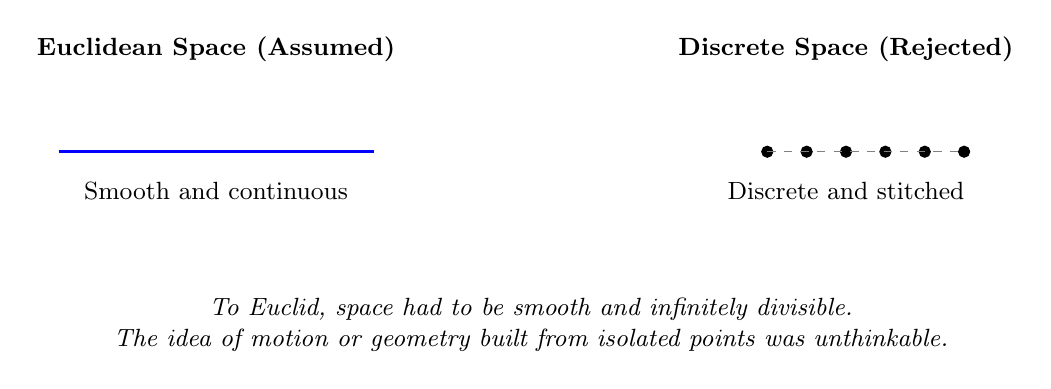
\begin{tikzpicture}[scale=1.0, every node/.style={font=\small}, >=stealth]

% Title labels
\node at (-4, 2.3) {\textbf{Euclidean Space (Assumed)}};
\node at (4, 2.3) {\textbf{Discrete Space (Rejected)}};

% Smooth line (left)
\draw[very thick, blue] (-6,1) -- (-2,1);
\node at (-4,0.5) {\small Smooth and continuous};

% Discrete line (right) - stitched points
\foreach \x in {-1, -0.5,...,1.5} {
    \filldraw[black] (\x + 4,1) circle (2pt);
}
\draw[dashed, gray] (3,1) -- (5.5,1);
\node at (4,0.5) {\small Discrete and stitched};

% Commentary below
\node[align=center] at (0, -1.2) {
    \textit{To Euclid, space had to be smooth and infinitely divisible.} \\
    \textit{The idea of motion or geometry built from isolated points was unthinkable.}
};

\end{tikzpicture}
\caption{Euclid assumed space was smooth—not made of discrete dots but of continuous lines and shapes. This allowed motion, geometry, and shape to make sense.}
\end{figure}

